\documentclass[10pt,twocolumn,letterpaper]{article}
\usepackage{cvpr}
\usepackage{graphicx}
\usepackage{amsmath}
\usepackage{amssymb}
\usepackage{booktabs}
\usepackage{tikz}
\usetikzlibrary{shapes.geometric, arrows}

\usepackage[pagebackref,breaklinks,colorlinks]{hyperref}
\usepackage[capitalize]{cleveref}
\crefname{section}{Sec.}{Secs.}
\Crefname{section}{Section}{Sections}
\Crefname{table}{Table}{Tables}
\crefname{table}{Tab.}{Tabs.}

\begin{document}

\title{Introducing Gender Stereotype-Aware Loss Regularizers to Reduce Gender-Based Bias in Language Models}

\author{Divyajeet Singh\\
{\tt\small divyajeet21529@iiitd.ac.in}
\and
Mehak Gopal\\
{\tt\small mehak21475@iiitd.ac.in}
\and
Siddhant Rai Viksit\\
{\tt\small siddhant21565@iiitd.ac.in}
\and
Sohum Sikdar\\
{\tt\small sohum20339@iiitd.ac.in}
}
\maketitle

\begin{abstract}
Deep learning-based natural language models are becoming increasingly capable of learning patterns in various languages.
Studies show that blind application of such models presents the risk of memorizing and amplifying the bias in the data on which they are trained.
Motivated by recent works in the field of ethics in artificial intelligence, we analyze the presence of gender bias in Masked Language Models (MLMs), specifically the BERT Masked Language Model.
This paper presents two novel loss regularizers to control and mitigate gender-related stereotypical bias in language models.
These regularizers can be used with regular MLM objectives, using which the MLM learns to eliminate bias in datasets by penalizing stereotypical predictions made by the model.
Using these approaches, we fine-tune the BERT MLM and quantitatively and qualitatively analyze the difference in predictions of the pre-trained and fine-tuned models.
\end{abstract}

%%%%%%%%% BODY TEXT
\section{Introduction}
\label{sec:intro}
In recent years, the proliferation of artificial intelligence, particularly in natural language processing, has catalyzed profound advancements.
However, these advancements have also given into the inherent biases encoded within these models, often reflecting and perpetuating societal biases and prejudices, which become more prominent as larger models are introduced and prepared using massive datasets.
Among the most concerning biases is gender bias, which manifests in language models through skewed representations and predictions, potentially reinforcing harmful stereotypes and inequities.

The prevalence of gender bias in deep learning-based natural language systems has gained attention from modern researchers.
Works such as Bolukbasi et al. \cite{biased-bert-embeddings}, Jentzsch et al. \cite{bias-measure}, and Bhardwaj et al. \cite{bert-bias-investiagion} have highlighted instances where models based on BERT (Bidirectional Encoder Representations from Transformers) exhibit gender-based biases, which potentially influence decisions in sensitive areas such as hiring, loan approval, and content recommendation.
Recognizing the ethical imperative to eliminate such biases, scholars strive to develop techniques that enforce fairness and inclusivity in these systems.

This paper presents two novel approaches to mitigate gender bias in BERT's Masked Language Model (MLM), a state-of-the-art pre-trained NLP model which has demonstrated remarkable performance across various NLP tasks.
Like many deep learning models, BERT is susceptible to encoding and perpetuating gender biases in its training data \cite{bert-bias-structure}.
Our proposed methodology addresses this concern by introducing two Gender Stereotype-Aware Loss Regularizers (Gals) designed to penalize predictions that exhibit gender bias during the fine-tuning process of BERT's MLM.
We show that incorporating the GAL Regularizers into the MLM training objective encourages the model to generate more gender-neutral predictions, thereby mitigating the amplification of gender bias in its outputs.
This results in a more gender-neutral model, obtained by targeting stereotypical model responses and reducing their prediction probabilities.

\section{Related Work}
\label{sec:relatedwork}

\subsection{\href{https://arxiv.org/abs/1607.06520}{Man is to Computer Programmer as Woman is to Homemaker? Debiasing Word Embeddings}}

Bolukbasi et al. \cite{biased-bert-embeddings} study the nature of BERT embeddings and discover that BERT word embeddings, even when fine-tuned on real-world datasets like Google News, exhibit a concerning amount of male/female stereotypes.
They showed that while the embeddings effectively capture the notion of gender using specific dimensions, they also pinpoint sexism implicit in the text.
As an interesting example, they observed that
\begin{align*}
    \textbf{man} - \textbf{woman} &\approx \textbf{king} - \textbf{queen} \\
    &\approx \textbf{computer programmer} - \textbf{homemaker}
\end{align*}
The embeddings seem to capture predominantly male and female occupations as stereotypical \textit{he}-\textit{she} analogies such as shopkeeper-housewife and surgeon-nurse, along with gender-appropriate analogies like brother-sister and ovarian cancer-prostate cancer along the same dimensions.
The paper focuses on the geometry and physical distributions of the embeddings and finds that along with the bias, the embedding space also contains information to help reduce the bias.

The authors study and identify the subspace of the embeddings that capture gender-based relationships and neutralize and equalize the space from gender-neutral words, ensuring that neutral words are equidistant from all words in each gendered set.
For example, the \textbf{babysit} would be equidistant to \textbf{grandfather} and \textbf{grandmother}.
This way, they present debiasing techniques to de-bias the embeddings geometrically while still preserving their most semantically meaningful properties.


\subsection{\href{https://arxiv.org/abs/2306.15298}{Gender Bias in BERT -- Measuring and Analysing Biases through Sentiment Rating in a Realistic Downstream Classification Task}}
Jentzsch \& Turan \cite{bias-measure} analyze the gender-based biases in multiple publicly available BERT models.
Their paper uses seven different publicly available BERT models in nine different training conditions (63 models in total) to analyze gender bias using the IMDB Large Movie Review Data.
They introduce a novel method to measure sentiment bias, where bias is defined as the difference in sentiment valuation of female and male sample versions.
Their bias measure is as follows:
\begin{align*}
    Bias_{XY}(i) &= \Delta \text{sent} \\
        &= sent(i_{Y}) - sent(i_{X})
\end{align*}
where, $X=Female$ and $Y=Male$. $Bias_{XY}(i)$ represents the bias for a sample $i$ with $X$ version as $i_{X}$ and $Y$ version as $i_{Y}$.
The experimental pipeline of this paper follows four major steps
\begin{enumerate}
    \item The IMDB data collected was preprocessed to remove all punctuation and lowercase.
    The dataset was labelled using a thresholding method.
    Reviews with ratings $\leq 4$ were labelled as negative, while those with $\geq 7$ were marked as positive.
    \item The sentiment classifiers were trained by fine-tuning seven common BERT models. Different sizes in the same architecture were also tested.
    \item These models were then tested on the manipulated test data.
    \item The results obtained were used to calculate the gender bias.
\end{enumerate}
They concluded and showed that all trained classifiers show significant gender bias and highlighted that the biases are propagated from underlying pre-trained BERT models rather than learnt in task-specific training.

\subsection{\href{https://aclanthology.org/2021.findings-emnlp.211/}{Collecting a Large-Scale Gender Bias Dataset for Coreference Resolution and Machine Translation}}
\label{subsec:dataset}

Levy et al. \cite{bug-dataset} presented BUG, a large-scale gender-bias evaluation corpus consisting of diverse, real-world scenarios.
Using this dataset, they evaluate gender bias on a large scale using machine translation and coreference resolution.
Upon fine-tuning a model on the BUG dataset, they were able to show that that model was less prone to make gender-biased predictions.

To make BUG, they used 14 lexical-syntactic patterns, with two main anchors, a pronoun and a profession, which the pattern indicates are co-referring.
To match these 14 patterns against real-world texts, they used SPIKE, which indexes large-scale corpora and retrieves matching instances given a lexical-syntactic pattern.
Each instance in BUG has also been marked as stereotypical, neutral or anti-stereotypical.
The results were all filtered with a predefined list of professions taken from the U.S. Census.

To evaluate their models, they used three main metrics
\begin{enumerate}
    \item Accuracy: The F1 score of the gender prediction.
    \item Population Bias ($\Delta G$): This denotes the difference in the accuracy between sentences with entities that co-refer with a masculine pronoun versus those with entities that co-refer with feminine pronouns.
    \item Historical Bias ($\Delta S$): This denotes the accuracy difference between stereotypical and anti-stereotypical sentences.
\end{enumerate}

Their results concluded that all tested models for machine translation and coreference resolution are prone to gender bias in real-world texts.
A spanBERT model, fine-tuned on the anti-stereotypical portion of BUG, yielded an error reduction of 50\% at the cost of an absolute 1\% drop in overall performance accuracy.

\section{Methodology}
\label{sec:methodology}
Our primary objective is to de-bias the BERT Masked Language Model.
While working on an unbiased sentiment analyser, we note that Jentzsch \& Turan \cite{bias-measure} perform gender masking on gendered tokens in their sentence.
This results in two masked versions of one original sentence - Male Masked and Female Masked.
We hypothesize that their masking strategy is sub-optimal, as they convert all gendered words into the same gender, thereby losing out on cross-gender relationships.
To tackle this, we present a unique flipping strategy - for each sentence in the corpus, we create its \textit{Gender Flipped} version by flipping all its gendered tokens.
Our strategies are compared in Figure \ref{fig:masking}
\begin{figure}
    \centering
    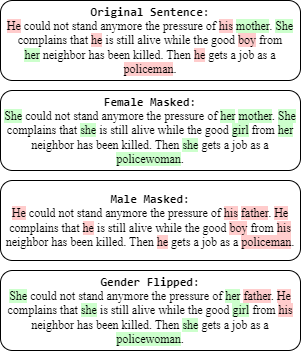
\includegraphics[width=0.45\textwidth]{Assets/masking.png}
    \caption{Masking and Flipping strategies for gendered sentences}
    \label{fig:masking}
\end{figure}

To create the Flipper, we used a public dictionary of gendered words in English, available at \href{https://github.com/ecmonsen/gendered_words}{\texttt{https://github.com/ecmonsen/gendered\_words}}.
The dictionary was created by manually tagging a large set of words as male, female, or neutral.
We form a frozen mapping of male-to-female and female-to-male correspondences using this dictionary.
For example, \texttt{actress} is mapped to \texttt{actor}, \texttt{brother} is mapped to \texttt{sister}, and so on.

The first GAL Regularizer can be used with the MLM objective of the BERT MLM, which is typically the Cross-Entropy Loss between the original sentence and its prediction after masking.
The regularizing term is introduced using the prediction of the flipped sentence.
Let $S_{O}$ be the original sentence and $S_{F}$ be its flipped version.
We create a mask which masks each token independently with probability $p$ and mask both sentences using it.
Let $L_{0}$ and $L_{F}$ be their corresponding predicted logits on the masked sentences.
Then, the final fine-tuning objective is given by
\begin{equation}
    \mathcal{L}_{1} = \textsc{CE}(S_{O}, L_{O}) + \lambda \ \textsc{Mse}(L_{O}, L_{F})
\end{equation}
The idea is to reduce the difference/\textit{distance} between the predictions for both the original and flipped sentences.
$\lambda$ is a hyperparameter to influence the strength of regularization.

The second GAL Regularizer can also be used with the MLM objective to create the final loss function.
This time, we mask all the gendered tokens in the sentence.
Then, we define the final fine-tuning objective as
\begin{equation}
    \mathcal{L}_{2} = \textsc{CE}(S_{O}, L_{O}) + \lambda \ \textsc{CE}(S_{F}, L_{O})
\end{equation}
The hope for this idea is to ensure that the model learns to predict both genders under appropriate contexts with approximately equal probability given any sentence.

Concisely, our contributions are two GAL regularizers
\begin{align}
    \textsc{Gal}_{1} &= \textsc{Mse}(L_{O}, L_{F}) \\
    \textsc{Gal}_{2} &= \textsc{CE}(S_{F}, L_{O})
\end{align}
which can be used appropriately with the MLM objective to de-bias the MLM's outputs.
The final model architectures are given in Figure \ref{fig:model1} and Figure \ref{fig:model2}.
\begin{figure}
    \centering
    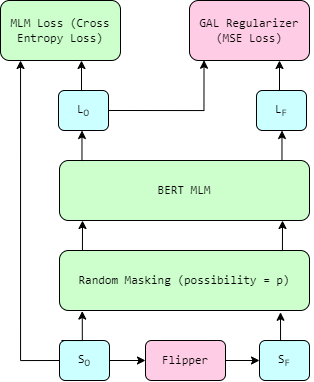
\includegraphics[width=0.4\textwidth]{Assets/model1.png}
    \caption{Model Architecture for fine-tuning with $\textsc{Gal}_{1}$}
    \label{fig:model1}
\end{figure}
\begin{figure}
    \centering
    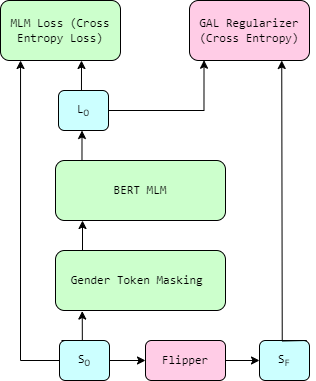
\includegraphics[width=0.4\textwidth]{Assets/model2.png}
    \caption{Model Architecture for fine-tuning with $\textsc{Gal}_{2}$}
    \label{fig:model2}
\end{figure}

One final idea is to use a randomized loss regularizer, $\textsc{Gal}_{R}$, in which we omit including the regularizer itself with some probability.
As per our experiments, we were motivated to only introduce this technique with $\textsc{Gal}_{2}$.
\begin{equation}
    \textsc{Gal}_{R} = \textbf{I}_{p} \ \textsc{Gal}_{2} = \textbf{I}_{p} \ \textsc{CE}(S_{F}, L_{O})
\end{equation}
where $\textbf{I}_{p} \sim \textsc{Bernoulli}(p)$ is a variable which switches to $1$ with probability $p$.
This way, with probability $1-p$, the model only uses the MLM loss for loss calculation, gradient propagation, and parameter updates.
This ideally ensures that the model does not throw away its already learned representations fast enough in the pursuit to minimize the regularizing term.

\section{Dataset}
Noticing the prevalence of gender-based bias in neural language models (specifically in machine translation and coreference resolution), Levy et al. \cite{bug-dataset} crafted a large-scale gender bias dataset called BUG.
The dataset was created with more than 105,000+ diverse real-world English sentences, including stereotypical gender roles like female nurses and non-stereotypical gender roles like male dancers.
The dataset is an unlabelled corpus of data relating to gender roles in society, which is perfect for our application.
For example, the dataset consists of sentences like \textit{"He was an American tap dancer, educator, and choreographer."} which are non-stereotypical, and sentences like \textit{"Her ballerina skills were unmatched, but still questioned by many."}.

The dataset was collected semi-automatically from different real-world corpora, designed to be challenging regarding societal gender role assignments using techniques strategized to combat stereotypes as discussed in the Literature Review in \ref{subsec:dataset}.
They used 14 lexical-syntactic patterns with two main anchors - a pronoun and a profession and performed co-reference resolution to indicate which anchors relate.
The dataset is complete with labels indicating whether each sentence in the corpus is stereotypical (+1), neutral (0), or anti-stereotypical (-1) and the professions and pronouns prevalent in the sentence.

The dataset is publicly available on GitHub, \texttt{\href{https://github.com/SLAB-NLP/BUG}{https://github.com/SLAB-NLP/BUG}}.

\subsection{Dataset Preparation and Preprocessing}
To suit our training pipeline, we simply utilize the unlabeled sentences.
We ignore the stereotype labels in the dataset as we must fine-tune our model on a balanced mix of neutral, stereotypical, and anti-stereotypical sentences.
Figure \ref{fig:distribution} displays the distribution of sentences in each class.
\begin{figure}
    \centering
    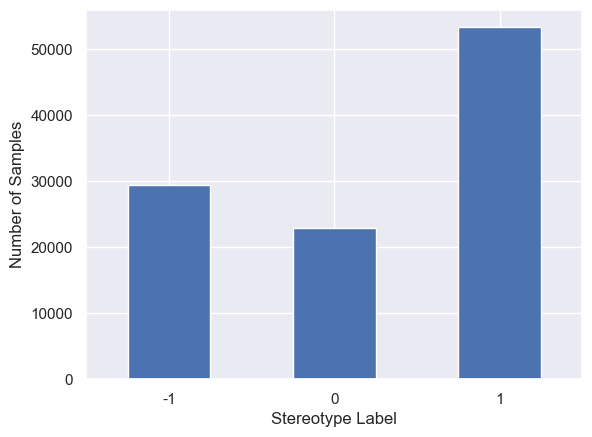
\includegraphics[width=0.45\textwidth]{Assets/distribution.png}
    \caption{Distribution of stereotype labels in BUG}
    \label{fig:distribution}
\end{figure}
Finally, we use the flipping strategy described in \ref{sec:methodology} to obtain the gender-flipped versions of each sentence.

\subsection{Alternate Datasets}
We also adopted an alternate strategy to extend the dataset.
Under this, we picked up large volumes of text corpora that we expected to be relevant to our problem statement.
Using our sentence gender flipper, we identify gendered sentences in the corpora and append them to our dataset.
However, a large fraction of the sentences were found to be irrelevant to the problem statement.
Corpora such as \href{https://huggingface.co/datasets/wikitext}{wikitext-103-v1} also contained gendered sentences relating to biology and botany.
Such sentences may hinder our progress as the model may lose discriminative ability against factual truths.
For example, it is known that pregnant male seahorses give birth to live young \cite{seahorse}.
Our training procedure may penalize the model for producing factually correct outputs.

\section{Experimental Setup}
We set up our experiments under the following constraints.
The pre-trained BERT MLM checkpoint, available through Hugging Face, and the BERT base uncased tokeniser were used for this task.
We used the Adam optimizer with a learning rate of $5e-5$ for all experiments, and the batch size was set to $16$.
The model was trained on A-100 GPUs.
We run the fine-tuning for a total of 3 epochs, as suggested by \cite{bert}.
Our experimental pipeline is shown in Figure \ref{fig:pipeline}.
\begin{figure}
    \centering
    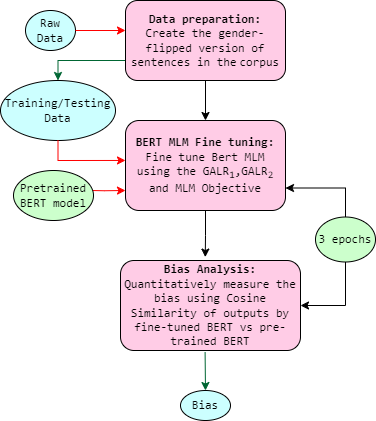
\includegraphics[width=0.45\textwidth]{Assets/pipeline.png}
    \caption{Experiment Pipeline}
    \label{fig:pipeline}
\end{figure}

To test $\textsc{Gal}_{1}$, we performed several experiments.
We tested regularizing strengths of $\lambda = 2e-5, 0.1, 1, 10, 100$.
We observed that with higher values of the regularizing strengths, the model prioritizes minimizing the gender loss term more than the MLM loss, resulting in meaningless outputs.
It tends to produce extremely neutral words for every predicted token, such as \texttt{the}, \texttt{and}, \texttt{on}, etc., entirely losing the sentence coherence.

To test $\textsc{Gal}_{2}$, we tested regularizing strengths of $0.5$ and $1$.
We found that with $\lambda = 1$, the model MLM is de-biased to the best possible extent.
However, we note that even in this case, the model invariably produces some outputs we cannot reason for.

Finally, the pre-trained BERT MLM was fine-tuned on the Randomized Ensemble Regularizer, $\textsc{Gal}_{R}$.
In the ensemble method of fine-tuning,
We observed that the hyperparameter setting of $\lambda = 1$ and $p = 0.5$ works well for our use case.
This way, we ensure that the MLM retains its most useful predictions while focussing on overcoming the bias.

\section{Results}
Our qualitative and quantitative analysis identifies the model fine-tuned with the $\textsc{Gal}_{R}$ regularizer as the best model.
We visualize the loss per step of the best model in Figure \ref{fig:loss}.
\begin{figure}
    \centering
    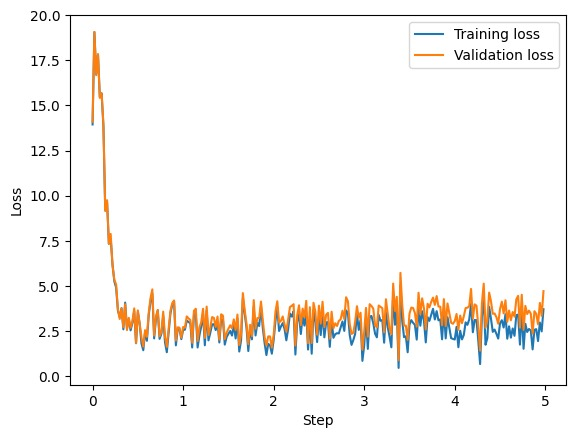
\includegraphics[width=0.5\textwidth]{Assets/loss.jpg}
    \caption{Loss per step of fine-tuning}
    \label{fig:loss}
\end{figure}

We first qualitatively assess the performance of our models.
We use a dataset by Nangia et al. \cite{test}, explicitly curated to analyze social biases in masked language models.
The dataset contains pairs of male and female-dominated sentences in professional and social environments.
It is publicly available at \href{https://github.com/nyu-mll/crows-pairs}{\texttt{https://github.com/nyu-mll/crows-pairs}}.
Consider a sentence from this dataset \texttt{"My [MASK] spent all day cooking food for dinner."}.
The predictions with probabilities are given in Table \ref{tab:probs}.
\begin{table}
    \centering
    \begin{tabular}{c|c|c}
         \textbf{Model} & \textbf{Word} & \textbf{Probability} \\
         \hline
         Pre-trained Base & \texttt{Mom} & 0.36 \\
         Pre-trained Base & \texttt{Mother} & 0.26 \\
         Pre-trained Base & \texttt{Dad} & 0.10 \\
         \hline
         $\textsc{Gal}_{1}$ & \texttt{Friend} & 0.22 \\
         $\textsc{Gal}_{1}$ & \texttt{Mother} & 0.12 \\
         $\textsc{Gal}_{1}$ & \texttt{Chef} & 0.10 \\
         \hline
         $\textsc{Gal}_{2}$ & \texttt{[PAD]} & 0.23 \\
         $\textsc{Gal}_{2}$ & \texttt{Mother} & 0.11 \\
         $\textsc{Gal}_{2}$ & \texttt{Father} & 0.08 \\
         \hline
         $\textsc{Gal}_{R}$ & \texttt{Mother} & 0.20 \\
         $\textsc{Gal}_{R}$ & \texttt{Father} & 0.12 \\
         $\textsc{Gal}_{R}$ & \texttt{Friend} & 0.08
    \end{tabular}
    \caption{Prediction Probabilities for the Test Sentence}
    \label{tab:probs}
\end{table}

To quantitatively analyze bias, we perform sentence similarity matching using cosine similarity.
On the test dataset, we calculate the cosine similarity between the predicted sentences for each original sentence and its flipped version.
We hypothesize that after the fine-tuning steps, the MLMs are de-biased enough to produce semantically meaningful yet similar outputs for both the original and gender-flipped sentences.
As the literature review suggests, the pre-trained BERT MLM simply produces varying outputs depending on gender-based context.
So, our final bias quantifier is
\begin{equation}
    \textsc{Bias}(M) = \frac{1}{N} \sum_{i=1}^{N} \textsc{Cos}\left( M\left( S_{O}^{(i)} \right), M\left( S_{F}^{(i)} \right) \right)
\end{equation}
where $S_{O}^{(i)}$ and $S_{F}^{(i)}$ are the original and flipped versions of the $i^{th}$ sentences, $M$ is the model, and $\textsc{Cos}$ represents the cosine similarity.
As opposed to just producing higher similarity scores, a sensible de-biased model must find a balance between producing an extremely high similarity and predicting meaningful outputs.
The test results are summarized in Table \ref{tab:cosine-sim}.
\begin{table}
    \centering
    \begin{tabular}{c|c}
         \textbf{Model} & \textbf{Cosine Similarity} \\
         \hline
         Pre-trained Base & $0.9522 \pm 0.0342$ \\
         $\textsc{Gal}_{1}$ & $0.9996 \pm 0.0005$ \\
         $\textsc{Gal}_{2}$ & $0.9976 \pm 0.0078$ \\
         $\textsc{Gal}_{R}$ & $0.9972 \pm 0.0077$
    \end{tabular}
    \caption{Cosine Similarity between Original and Flipped Sentences}
    \label{tab:cosine-sim}
\end{table}

We find that the model fine-tuned on the probabilistic regularizer $\textsc{Gal}_{R}$, produced the most semantically meaningful and gender-neutral outputs.

\section{Discussion}
Through the strategies presented in this paper, we aim to work towards a lingering issue in all of machine learning, especially in the natural language field.
We hope the ideas shared in this paper spark further discussion and interest in the intersection of gender studies and natural language processing since all models must represent all groups fairly.
The problem is simple - biased data will produce biased models.
Its solution, however, turns out to be tricky.

\subsection{Limitations}
Our methodology revolves around \textit{flipping} the gendered words in sentences and analyzing and de-biasing the model results.
However, the ideas in this paper may turn back on themselves if proper datasets are not used for fine-tuning.
For example, if one chooses to fine-tune for gender-based bias minimization using our technique with a dataset of fauna information, such as a subset of the Wikitext, the models may lose their discriminative ability towards biological truths.

\subsection{Possibilities for Exploration}
Since the regularizers work favourably, we hypothesize that even more representative datasets can boost the performance we intend to achieve.
For example, the \href{https://huggingface.co/datasets/bookcorpus}{bookcorpus} dataset from Hugging Face, a corpus of text from the book, contains more than 74 million entries, which must embody the sexism present in conservative written literature.
Such large datasets are well-suited to the problems we intend to solve.

\section{Conclusion and Future Work}
Through this paper, we have introduced two novel Gender-Stereotype Aware Loss Regularizers.
We have demonstrated how incorporating these regularizers in the training objective of the Masked Language Models reduces gender-based bias and favours the model to produce more gender-neutral outputs while remaining semantically meaningful under appropriate contexts.
We show that the BERT-based masked language model when fine-tuned using the randomized GAL regularizer, results in the most gender-neutral model.

We believe the same idea can be transferred from Masked Language Modeling to the Next Sentence Prediction Problem.
Next sentence predictors, even those trained on humongous datasets, are prone to gender-based bias due to the bias inherent to their training datasets.
This is due to the very nature of societal bias - larger datasets amplify them \cite{bias}.
Hence, we propose a technique to de-bias GPT-2 as a future plan.
The basic model architecture is shown in Figure \ref{fig:future}.
\begin{figure}
    \centering
    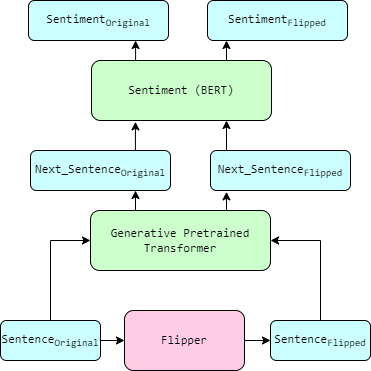
\includegraphics[width=0.45\textwidth]{Assets/future_model.png}
    \caption{Proposed model architecture to de-bias GPT-2}
    \label{fig:future}
\end{figure}
The basic low-level idea is to generate the next sentence from the original and gender-flipped versions of the sentences in the corpus and perform sentiment-based matching of the outputs.
This sentiment matching can then act as a regularizing term, where we hope to produce sentences with similar sentiments for either version of the sentence.
We may also use metrics such as cosine similarity to perform a matching.

{\small
\bibliographystyle{ieee_fullname}
\bibliography{egbib}
}

\end{document}
